This chapter outlines the theoretical and mathematical concepts of the high energy particle physics.
The Standard Model of particle physics (SM)~\cite{BF02726525,Glashow,PhysRevLett.19.1264,Herrero:1998eq,CBO9780511791406} is developed since the early 1970s and it has successfully explained almost all experimental results.
The SM is a well-tested and the most successful physics theory to describe the nature of the elementary particles and their interactions.
An overview of the SM is given in Section~\ref{sec:sm}.
After that, an emphasis on the electroweak interactions of the SM is discussed in Section~\ref{sec:ewk}.

%%%
%%%
%%%

\section{The Standard Model of Particle Physics}
\label{sec:sm}
The Standard Model of particle physics is known as the most accurate theory for describing the elementary particles and the interactions between them.
By combining the quantum mechanics and special relativity, the SM is a relativistic \textit{quantum field theory} (QFT) based on a $SU(3)_{C} \otimes SU(2)_{L} \otimes U(1)_{Y}$ symmetry gauge group, where $C$ denotes color, $L$ represents left chirality, and $Y$ stands for weak hypercharge, respectively.
The $SU(3)_{C}$ group is the basis for \textit{Quantum Chromodynamics} (QCD) which describs the strong interaction and the $SU(2)_{L} \otimes U(1)_{Y}$ group is the fundation of the electroweak interaction which unifies the electromatnetic and weak interactions.
Therefore, the SM Lagrangian is invariant under the local gauge transformation.
According to \textit{Noeher's Theorem}~\cite{00411457108231446}, the invariance of an action of a physical system undergoes a symmetry transformation corresponding to a conservation law and vice versa. 
The gauge invariance of the SM Lagrangian corresponds to the conserved quantum numbers, or the charges, of each interaction.
The conserved charges are the three color charge (red, blue, green) for the strong interaction, the third component of the weak isospin $I_{3}^{W}$ for the weak interaction, and the electric charge $Q$ for the electromagnetic interaction.

%%%
%%%
%%%

\subsection{Particle Content}
\label{subsec:sm_particle_content}
According to the SM, all matter around us is made of elementary particles called \textit{quarks} and \textit{leptons}.
The quarks and leptons are called fermions which have half integral spin $s=\frac{1}{2}$, hence the fermions follow the Pauli exclusion principle which says no two fermions have the same quantum state at the same time.
Each fermion has an anti-fermion with the equal mass but carries opposite electric charge, weak isospin and color charge.
There are six quarks and six leptons, they are group into three paris, or "\textit{generations}", ordered by their mass.
The lightest and most stable particles constitute the first generation and they are constituents of ordinary matter.
The heavier and less stable particles form the second and third generations and the heavier particles quickly decay to the next most stable particles.
The three generations of quarks are up ($u$) and down ($d$), charm ($c$) and strange ($s$), and top ($t$) and bottom ($b$) quarks.
The up-type quarks ($u, c, t$) carry $+\frac{2}{3}|e|$ charge and with isospin $+\frac{1}{2}$ while the down-type quarks ($d, s, b$) carry $-\frac{1}{3}|e|$ charge with isospin $-\frac{1}{2}$.
The quarks carry an additional color charge of either red, green, or blue, and hence they only interact via the strong force.
Because the strong force holds quarks together, only non-integer charges of the quark combinations are experimentally allowed.
The quark combinations are called \textit{hadrons} which can be categorised into \textit{mesons} and \textit{baryons}.
The meson is composed by a quark and anti-quark pair ($q\bar{q}$) whereas the baryon is made up by three quarks ($qqq$ or $\bar{q}\bar{q}\bar{q}$).
Only colorless bound states of hadrons are allowed so the quark and anti-quark pair in a meson should contain color and anti-color and the three quarks in a baryon must carry different colors.
The leptons are colorless and are therefore participating in the weak and electromagnetic force only. 
They do not participate in the strong interaction.
The electron-type leptons ($e, \mu, \tau$) carry an elementary charge $|e|$ and their corresponding neutrinos ($\nu_{e}, \nu_{\mu}, \nu_{\tau}$) are neutral.
The neutrinos have very little mass and interact via weak force only.
A summarized table of the properties of quarks and leptons is given in Table~\ref{tab:sm_fermions}.

\begin{table}[htp]
%\begin{center}
\resizebox{\textwidth}{!}{% <------ Don't forget this %
\begin{tabular}{cccccccc}
\hline
\hline
Generation & Fermion & & particle & electric charge $Q$ & weak isospin $I_{3}$ & color charge $C$ & mass [{\GeV}]\\
\hline
\multirow{4}{*}{I} & \multirow{2}{*}{Quark}  & $u$       & up quark          & $+\frac{2}{3}|e|$ & $+\frac{1}{2}$ & r,g,b & 0.0023\\
                   &                         & $d$       & down quark        & $-\frac{1}{3}|e|$ & $-\frac{1}{2}$ & r,g,b & 0.0048\\
                   & \multirow{2}{*}{Lepton} & $e$       & electron          & $-1|e|$           & $-\frac{1}{2}$ & -     & 0.00051\\
                   &                         & $\nu_{e}$ & electron neutrino & 0                 & $+\frac{1}{2}$ & -     & $< 2 \times 10^{-9}$\\
\hline
\multirow{4}{*}{II} & \multirow{2}{*}{Quark}  & $c$         & charm quark   & $+\frac{2}{3}|e|$ & $+\frac{1}{2}$ & r,g,b & 1.275\\
                    &                         & $s$         & strange quark & $-\frac{1}{3}|e|$ & $-\frac{1}{2}$ & r,g,b & 0.095\\
                    & \multirow{2}{*}{Lepton} & $\mu$       & muon          & $-1|e|$           & $-\frac{1}{2}$ & -     & 0.106\\
                    &                         & $\nu_{\mu}$ & muon neutrino & 0                 & $+\frac{1}{2}$ & -     & $< 1.9 \times 10^{-7}$\\
\hline
\multirow{4}{*}{III} & \multirow{2}{*}{Quark}  & $t$          & top quark    & $+\frac{2}{3}|e|$ & $+\frac{1}{2}$ & r,g,b & 173.2\\
                     &                         & $b$          & bottom quark & $-\frac{1}{3}|e|$ & $-\frac{1}{2}$ & r,g,b & 4.18\\
                     & \multirow{2}{*}{Lepton} & $\tau$       & tau          & $-1|e|$           & $-\frac{1}{2}$ & -     & 1.777\\
                     &                         & $\nu_{\tau}$ & tau neutrino & 0                 & $+\frac{1}{2}$ & -     & $< 1.82 \times 10^{-5}$\\

\hline
\hline
\end{tabular}
}
%\end{center}
\caption{The SM fermions with charges and masses~\cite{PDG}.}
\label{tab:sm_fermions}
\end{table}%

%\begin{figure}[htbp]
%\begin{center}
%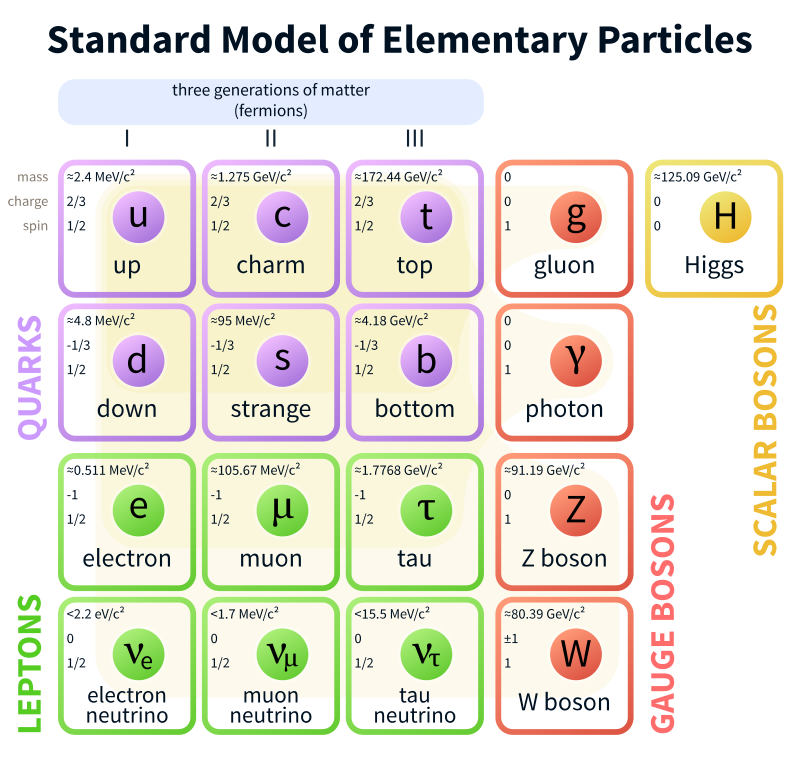
\includegraphics[scale=0.3]{800px-Standard_Model_of_Elementary_Particles.png}
%\caption{default.
%https://en.wikipedia.org/wiki/Standard_Model
%}
%\label{fig:sm_particles}
%\end{center}
%\end{figure}

%%%
%%%
%%%

Three of the four fundamental forces, strong, weak, electromatnetic forces are parts of the SM now and the gravitational fources could not yet be included in the SM.
Table~\ref{tab:fundamental_forces} shows the four fundamental forces, the relative strength and range together with the theories and the mediators.

\begin{table}[htp]
\begin{center}
\begin{tabular}{ccccc}
\hline
\hline
Force & Rel. Strength & Range (m)& Theory & Mediator\\
\hline
Strong & $10$ & $10^{-15}$ & Chromodynamics & Gluon\\
Weak & $10^{-13}$ & $10^{-18}$ & Flavourdynamics & $W^{\pm}$ and $Z^{0}$ bosons\\
Electromagnetic & $10^{-2}$ & $\infty$ & Electrodynamics & Photon\\
\hline
Gravitational & $10^{-42}$ & $\infty$ & General relativity & Graviton\\
\hline
\hline
\end{tabular}
\end{center}
\caption{The four fundamental forces with the relative strength, interaction range, describing theory, and the mediator.}
\label{tab:fundamental_forces}
\end{table}%

%%%
%%%
%%%

























% Forces and carrier particles

% There are four fundamental forces at work in the universe: the strong force, the weak force, the electromagnetic force, and the gravitational force. They work over different ranges and have different strengths. Gravity is the weakest but it has an infinite range. The electromagnetic force also has infinite range but it is many times stronger than gravity. The weak and strong forces are effective only over a very short range and dominate only at the level of subatomic particles. Despite its name, the weak force is much stronger than gravity but it is indeed the weakest of the other three. The strong force, as the name suggests, is the strongest of all four fundamental interactions.
% Three of the fundamental forces result from the exchange of force-carrier particles, which belong to a broader group called “bosons”. Particles of matter transfer discrete amounts of energy by exchanging bosons with each other. Each fundamental force has its own corresponding boson – the strong force is carried by the “gluon”, the electromagnetic force is carried by the “photon”, and the “W and Z bosons” are responsible for the weak force. Although not yet found, the “graviton” should be the corresponding force-carrying particle of gravity. The Standard Model includes the electromagnetic, strong and weak forces and all their carrier particles, and explains well how these forces act on all of the matter particles. However, the most familiar force in our everyday lives, gravity, is not part of the Standard Model, as fitting gravity comfortably into this framework has proved to be a difficult challenge. The quantum theory used to describe the micro world, and the general theory of relativity used to describe the macro world, are difficult to fit into a single framework. No one has managed to make the two mathematically compatible in the context of the Standard Model. But luckily for particle physics, when it comes to the minuscule scale of particles, the effect of gravity is so weak as to be negligible. Only when matter is in bulk, at the scale of the human body or of the planets for example, does the effect of gravity dominate. So the Standard Model still works well despite its reluctant exclusion of one of the fundamental forces.
% So far so good, but...

% ...it is not time for physicists to call it a day just yet. Even though the Standard Model is currently the best description there is of the subatomic world, it does not explain the complete picture. The theory incorporates only three out of the four fundamental forces, omitting gravity. There are also important questions that it does not answer, such as “What is dark matter?”, or “What happened to the antimatter after the big bang?”, “Why are there three generations of quarks and leptons with such a different mass scale?” and more. Last but not least is a particle called the Higgs boson, an essential component of the Standard Model.
% On 4 July 2012, the ATLAS and CMS experiments at CERN's Large Hadron Collider (LHC) announced they had each observed a new particle in the mass region around 126 GeV. This particle is consistent with the Higgs boson but it will take further work to determine whether or not it is the Higgs boson predicted by the Standard Model. The Higgs boson, as proposed within the Standard Model, is the simplest manifestation of the Brout-Englert-Higgs mechanism. Other types of Higgs bosons are predicted by other theories that go beyond the Standard Model.
% On 8 October 2013 the Nobel prize in physics was awarded jointly to François Englert and Peter Higgs "for the theoretical discovery of a mechanism that contributes to our understanding of the origin of mass of subatomic particles, and which recently was confirmed through the discovery of the predicted fundamental particle, by the ATLAS and CMS experiments at CERN's Large Hadron Collider."
% So although the Standard Model accurately describes the phenomena within its domain, it is still incomplete. Perhaps it is only a part of a bigger picture that includes new physics hidden deep in the subatomic world or in the dark recesses of the universe. New information from experiments at the LHC will help us to find more of these missing pieces.
